\chapter{Auswertung}

In diesem Kapitel wird analytisch auf die vorangegangenen Resultate eingegangen und die Schwellenbestimmung der Rater und Software in evaluiert. Vorweg wird erläutert, welche Methoden genutzt wurden, um Messfehler vor der Auswertung zu detektieren um die Grafiken dementsprechend differenzierter zu interpretieren.

\section{Plausibilitätsprüfung der Messwerte}

Für die Spiroergometrie existieren keine validen Methoden zur Plausibilitätskontrolle der Messwerte. Empfohlen wird stattdessen zur groben Abschätzung der Vergleich von \acs{VE}-, \acs{VO2}- und Belastungszunahme, da zwischen diesen Parametern bis zum Erreichen der VT1 eine gewisse physiologische Proportionalität besteht. Für diese Abschätzung sollen zwei Faustformeln in der klinischen Spiroergometrie nutzbar sein, wobei $n$ die Anzahl der gefahrenen Stufen sei~\cite{Ruehle.2012}:
%
\begin{flalign}
\dot{V}E_{max}\hspace{1mm} \text{in \si{\litre\per\minute}} &= \SI{9}{\litre\per\minute} + n * \SI{9}{\litre\per\minute} \pm 10 \%
\label{eq:formel14}\\[1em]
\dot{V}O_{2max}\hspace{1mm} \text{in \si{\milli\litre\per\minute}} &= 5 * \left\lbrace m\right\rbrace \text{in \kilogram} * W_{max}\hspace{1mm} \text{in \watt} * \SI{10}{\milli\litre\per\minute} \pm 10 \%
\label{eq:formel15}
\end{flalign}
%
\acs{VE} und \acs{VO2} sollen demnach einen idealerweise linearen Verlauf über die Leistung annehmen. Da die Berechnungen jedoch kaum anthropometrischen Daten oder individuellen Trainingszustände einbeziehen, wurde auf die mathematische Art der Überprüfung wegen der großen Varianz an Trainingszuständen in dieser Arbeit verzichtet. Allerdings kann mithilfe eines grafischen Vergleichs der Parameter der Verlauf einer Messung analysiert und bewertet werden.\\
Abb. \ref{pic:pic15} in Kapitel 3.1.1 zeigt in Feld 5 und 6 einen solchen Messverlauf für die \acs{VE} und \acs{VO2} im Falle der Probandin 6w. In Ruhe beträgt die \acs{VE} ca. \SI{9}{\litre\per\minute}, steigt danach tatsächlich um ca. \SI{9}{\litre\per\minute}, doch danach flacht die Steigung ein wenig ab. Dennoch steigen die Graphen stetig an, weswegen von einem guten Messverlauf ausgegangen wird. Nicht bei allen Probanden jedoch hatten die Plots eine solche Form.\\
In Abb. \ref{pic:pic21} sind Plots mit Artefakten zu sehen. Zwischen den Stufen 2 und 6 schwanken die Messwerte sowohl für die \acs{VE}, als auch für die \acs{VO2} sehr stark. Es sind mehrere Abfälle des Graphen an Stelle eines stetigen Anstiegs sichtbar. Da die \acs{VO2} mathematisch von der \acs{VE} abhängt (vgl. Kapitel 1.2.1), ist von einem Messfehler der \acs{VE} auszugehen. Diese ist abhängig vom Atemzugvolumen sowie der \acs{AF}. Da auch diese beiden Parameter physiologisch bedingt ansteigen, ist es sehr wahrscheinlich, dass während der Messungen zwischen den betroffenen Stufen weniger Atemzüge korrekt erfasst wurden. Dies kann beispielsweise daran liegen, dass Probleme mit dem Mundstück bestanden. 7 der 28 Probanden empfanden die Ergonomie des Mundstücks als unangenehm und deuteten nach dem Test an, dass dieses die Atmung gerade zu Beginn einer Messphase erschwert habe.\\
Auch Proband 21m hatte Schwierigkeiten mit dem Mundstück und konnte dieses in mehreren Stufen nicht rechtzeitig für eine korrekte Atemzugerfassung platzieren. Einer weiteren Probandin rutschte das Mundstück bei erhöhter Belastung während einer Messung mehrmals aus dem Mund. Somit konnten die Graphen Aufschluss über den Erfolg einer Messphase zwischen zwei Stufen geben und bei der Analyse der restlichen Graphen zur Schwellenbestimmung unterstützen. Zum Beispiel konnten die Messpunkte der Atemäquivalente im 2. Feld der 6-Felder-Grafik direkt mit dem \acs{VE}/Watt-Plot verglichen und so verifiziert werden.\\
In Abb. \ref{pic:pic21} ist beispielsweise zu sehen, dass auch in den vier Feldern zur Schwellenbestimmung die Kurven zwischen positivem und negativem Verlauf schwanken. Im V-Slope in Feld 1 sinken die \acs{VO2} und \acs{VCO2} zwischen Messpunkt 3 und 4 sowie 4 und 5 wieder ab. Dies trifft auch auf die \acs{VE} und \acs{VCO2} in Feld 4 zu. Analog dazu sinkt die \acs{VE} im 5. Feld. Derartige Artefakte können mit der Mundstück-Problematik belegt werden, da die Messzeit mit \SI{30}{\second} gleichbleibend war. Durch den Verlust des Mundstücks innerhalb einer Messung wird auch die Anzahl der registrierten Atemzüge reduziert, sodass die Berechnung der \acs{AF} und \acs{VE} durch die Software fehlerhaft und der Durchschnitt im Gesamtverlauf stark beeinflusst wird.\\
In Feld 2 von Abb. \ref{pic:pic21} fällt bei Betrachtung der blauen \acs{EQO2}-Kurve auf, dass der Tiefpunkt sehr spät nach der 5. Stufe auftrat. Vergleicht man die Kurven mit Feld 5 und 6, kann auch dies durch Messfehler begründet werden, da auch in der 5. Stufe wieder ein Abfall der \acs{VE} beobachtet werden kann. Diese Plots wurden schließlich bei der Evaluierung der Ergebnisse berücksichtigt, um Unterschiede zwischen den Ratern und der Software zu erörtern und nachträglich diskutieren zu können, welche charakteristischen Punkte in den Plots tatsächlich durch die pathophysiologischen Veränderungen der Respiration und Ventilation bedingt waren.

\section{Evaluierung der Schwellenbestimmung}

Die Plots wurden bezüglich ihrer Qualität zunächst eigenständig und subjektiv in die Kategorien Gut und Kritisch einsortiert. Plots, die händisch mithilfe einer einzelnen Methode einfach auszuwerten waren und außerdem keine schwerwiegenden Artefakte aufwiesen, wurden als gut deklariert. In die Rubrik Kritisch kamen jene Graphen, die beispielsweise unregelmäßige Kurvenverläufe aufwiesen und dadurch nur sehr differenziert evaluiert werden konnten.
%
\begin{table}[H]
	\begin{center}
		\caption{Kategorisierung der Plots nach Qualität}
		\medskip
		\begin{tabulary}{\textwidth}{L L C C}
			\toprule
			& & Gut & Kritisch \\
			\midrule
			\midrule
			\multirow{3}{1.5cm}{\textbf{VT1}} & V-Slope & 7 & 21 \\
			& \acs{EQO2} & 13 & 15 \\
			\cmidrule{2-4}
			& \textsl{Summe} & 20 (36 \%) & 36 (64 \%) \\
			\midrule
			\multirow{3}{1.5cm}{\textbf{VT2}} & \acs{EQCO2} & 21 & 7 \\
			& \acs{VE}/\acs{VCO2} & 15 & 13 \\
			\cmidrule{2-4}
			& \textsl{Summe} & 36 (64 \%) & 20 (36 \%) \\
			\bottomrule
		\end{tabulary}
		\label{tab:tabelle7}
	\end{center}
\end{table}
%
Tab. \ref{tab:tabelle7} zeigt die Kategorien und Zuordnungen. Die jeweilige Menge an Graphen wurde in die zwei Spalten Gut und Kritisch eingeordnet. Da für jedes Messergebnis zwei neue Methoden angewandt wurden, waren insgesamt 56 Graphen je Schwelle auszuwerten. Mit 64 ~\% wurde der Großteil aller Plots zur Bestimmung der VT1 als kritisch bewertet. 36 ~\% wurden als gut eingestuft. Für die VT2-Bestimmung hingegen waren 64 ~\% der Graphen gut und 36 ~\% kritisch. 

\subsection{Evaluierung der VT1}

\subsubsection{Gute Ergebnisse}

Mit 20 von insgesamt 56 Plots für die VT1-Bestimmung konnte diese gut detektiert werden. Bei differenzierbaren V-Slopes, wie beispielsweise in Abb. \ref{pic:pic15} sichtbar, konnte der \acs{VCO2}-Anstieg optisch abgelesen werden. Dieselbe Abbildung zeigt auch eine gut auszuwertende \acs{EQO2}-Kurve. Diese steigt nach dem Tiefpunkt nach der 2. Stufe stetig an, sodass die VT1 relativ eindeutig bestimmt werden konnte. Abb. \ref{pic:pic17} enthält die algorithmisch bestimmten Schwellen für die Probandin. Aus den zwei Netzdiagramm in Abb. \ref{pic:pic22} ist zu entnehmen, dass Rater und Software anhand eines solchen Plots zu vergleichbaren Ergebnissen kamen.\\
\clearpage
In Abb. \ref{pic:pic19} ist erkennbar, dass der V-Slope zwar differenzierbar ist, aber durch die vielen Messpunkte geglättet wird und die Abstände zwischen einzelnen Punkten teilweise sehr klein wurden. Hier wich gemäß Abb. \ref{subpic:pic1} die VT1 nach Rater 1 von der nach Rater 2 und Software ab. Die \acs{EQO2}-Methode führte jedoch zu vergleichbaren VT1-Werten. Auch hier war der Tiefpunkt der \acs{EQO2}-Kurve relativ gut zu identifizieren.

\subsubsection{Kritische Ergebnisse}

Größtenteils war die VT1-Bestimmung anhand der vorliegenden Grafiken gemäß der Tab. \ref{tab:tabelle7} jedoch erschwert. Drei Viertel der V-Slope-Graphen wurden vorweg als kritisch eingestuft. Dies lag daran, dass die rein subjektive Identifizierung des ersten überproportionalen Anstiegs der \acs{VCO2} anhand von Mittelwerten dann schwierig war, wenn die V-Slopes und die zugeordneten \acs{HF}-Kurven nicht differenzierbar waren, wie beispielsweise ist den Plots in Abb. \ref{pic:pic16} und Abb. \ref{pic:pic18}. Diese Problematik trat relativ häufig auf und wurde auch vom 2. Rater moniert. Das Netzdiagramm in Abb. \ref{subpic:pic1} verdeutlicht, wie stark sich die Auswertungen der Rater und der Software dadurch unterscheiden. Rater 1 und Rater 2 kamen häufig zu ungleichen Ergebnissen beim V-Slope. Es ist im durch viele hellrote Schraffuren im Diagramm zu erkennen, dass der 2. Rater die VT1 meistens später bzw. bei höheren \acs{HF} bestimmte.\\
Zwei Beispiele hierfür sind die Probanden 8m sowie 21m. In Abb. \ref{pic:pic18} für 8m ist ein nicht differenzierbarer V-Slope zu sehen, der mehrere Knickpunkte enthält. Eine Vielzahl an solchen Punkten begünstigt eine große Varianz an Werten für die VT1. Während Rater 1 den ersten Anstieg in der 2. Stufe beobachtete, wurde er laut Rater 2 erst nach den Schwankungen der Werte in Stufe 6 erkennbar. Dasselbe Ergebnis entstand mit dem \acs{EQO2}. Der Tiefpunkt der \acs{EQO2}-Kurve liegt in Abb. \ref{pic:pic18} erst zwischen Stufe 6 und 7. Hier bestimmte Rater 2 dementsprechend auch die VT1. Da allerdings an diesem Punkt auch die \acs{EQCO2}-Kurve ansteigt und ein sehr leichter Anstieg der \acs{EQO2}-Kurve bereits nach Stufe 2 auftritt, wo das \acs{EQCO2} noch nicht zunimmt, wurde die VT1 von Rater 1 und auch von der Software dort identifiziert. Diese \acs{EQO2}-Steigung kann nachträglich mithilfe des \acs{VO2}/Watt-Plots in Feld 6 erörtert werden. Zwischen der 2. und 3. Stufe fällt die \acs{VO2} stärker ab, als die \acs{VE}. Nach Formel \eqref{eq:formel8} bedeutet dies, dass \acs{EQO2} einen größeren Wert annimmt und vom vorangehenden Wert somit ansteigt. Tab. \ref{tab:tabelle3} kann entnommen werden, dass Proband 8m ein junger Mann ist und mit ca. 13 Stunden Sport pro Woche einen wahrscheinlich sehr guten Trainingszustand besitzt. Dies berücksichtigend, kann die VT1 deutlich später angenommen werden und sich eher mit dem Ergebnis von Rater 2 decken.\\
Ein weiteres Beispiel einer solchen Differenz zwischen den Ratern liegt bei Proband 21m vor (siehe Abb. \ref{subpic:pic2}). Erneut kann diese durch die Schwankungen des \acs{EQO2} in Abb. \ref{pic:pic21} begründet werden. Rater 1 und Software nahmen hier auch den ersten \acs{EQO2}-Anstieg als die VT1 an, während Rater 2 die Schwelle am tatsächlichen Tiefpunkt der Kurve bestimmte. Beim V-Slope dieses Probanden fiel das Ergebnis anders aus und Rater 2 und Software kamen zu vergleichbaren Ergebnissen, obgleich Rater 1 die VT1 auch hier beim ersten \acs{VCO2}-Anstieg setzte.\\
Ein drittes kritisches Beispiel wird im Falle von 12m vorgestellt. Hier bestimmte die Software mit beiden Methoden die VT1 früher als die Rater. Bei Betrachtung von Abb. \ref{pic:pic20} fällt auf, dass die Kurvenverläufe allgemein recht eben sind. Anhand des V-Slopes fiel es beiden Ratern schwer, zu bestimmen, an welchem Punkt der Anstieg der \acs{VCO2} deutlich sichtbar war. Hier wird ein Vorteil der algorithmischen Auswertung deutlich, da die Software die größte Steigungsänderung mathematisch und daher eindeutig bestimmt. Im 2. Feld tritt erneut die Problematik mit dem späten Tiefpunkt der \acs{EQO2}-Kurve in Verbindung mit einem Knickpunkt der \acs{VO2}/Watt-Kurve auf, weshalb die Rater die VT1 dort später bestimmten. Bei vielen Plots musste differenziert werden, welcher Punkt der \acs{EQO2}-Kurve als \acs{POW} und damit als VT1 bezeichnet werden kann.\\
Letztlich zeigen die behandelten Beispielplots und die Diagramme in Abb. \ref{pic:pic23} und \ref{pic:pic24}, dass die Ergebnisse häufiger stark differieren und oftmals kein eindeutiger Bereich für die VT1 mittels V-Slope und \acs{EQO2} bestimmt werden kann. Die Ergebnisse beider Methoden weisen jeweils eine \acs{SD} von $\pm$14 \si{\per\minute} auf. Die gemittelte Differenz zwischen Ratern und Software fällt bei der \acs{EQO2}-Methode größer aus, was an zwei sehr großen Differenzen mit \SIlist{46,50}{\per\minute} liegt, die den Gesamtdurchschnitt bei 28 Probanden stark beeinflussen. Aus den gemittelten Werten für die VT1 der Rater und der algorithmischen Bestimmung wurden die Korrelationskoeffizienten r für den V-Slope und das \acs{EQO2} berechnet:
%
\begin{flalign*}
r_{V-Slope} = 0,526  &\hspace{2cm} r_{EQO_2} = 0,464
\end{flalign*}
%
Die beiden Werte liegen relativ mittig von null und eins und belegen somit, dass die algorithmischen sowie durch Rater bestimmten VT1 der Testmessungen aufgrund der häufig starken Differenzen nur bedingt korrelieren und die verwendeten Methoden dementsprechend mit dieser Art der Durchführung einer Leistungsdiagnostik nicht als optimal bezeichnet werden können.

\subsection{Evaluierung der VT2}

\subsubsection{Gute Ergebnisse}

Bei den Werten für die VT2 differieren die Ergebnisse deutlich weniger, wie Abb. \ref{pic:pic25} andeutet. Am erfolgreichsten fiel die VT2-Bestimmung mittels \acs{EQCO2}-Anstieg aus, was mit Abb. \ref{subpic:pic3} belegt werden kann. Lediglich bei fünf Probanden können Differenzen >\SI{10}{\per\minute} beobachtet werden (siehe Abb. \ref{pic:pic26}). Dabei bestimmte die Software die VT2 meistens ein wenig später als die Rater, was an hellgrünen Schraffuren in Abb. \ref{pic:pic25} zu erkennen ist. Erklären lässt sich dies z.B. anhand von Abb. \ref{pic:pic18} bei Proband 8m. Hier sind Schwankungen der \acs{EQCO2}-Steigung zu sehen, sodass die Kurve im letzten Drittel der Messung sogar zweimal ansteigt und zwischendurch einmal abfällt. So kam es zu unterschiedlichen Schwellen bei der manuellen Betrachtung durch die Rater.\\
Im Beispiel vom Probandin 6w in Abb. \ref{pic:pic17} ist sichtbar, dass die \acs{EQCO2}-Kurve stetig ansteigt. Rater 1 nahm die VT2 bereits beim ersten zeitlichen Anstieg nach Stufe 5 an. Software sowie Rater 2 wählten erst den überproportionalen Anstieg des \acs{EQCO2} nach Stufe 7 als die VT2. Die algorithmische Bestimmung erfolgt nach mehreren Schleifen, in denen Ausreißer bei der Steigung sowie die Referenzwerte der HUNT 3 Studie abgeglichen werden. Dieser Abgleich sorgt dafür, dass gelegentlich nicht der absolut erste \acs{EQCO2}-Anstieg markiert wird. Abb. \ref{pic:pic26} zeigt jedoch deutlich, dass große Differenzen zwischen den Instanzen recht selten sind und die Ergebnisse im Gesamtbild am meisten miteinander korrelieren.

\begin{figure}[H]
	\centering
	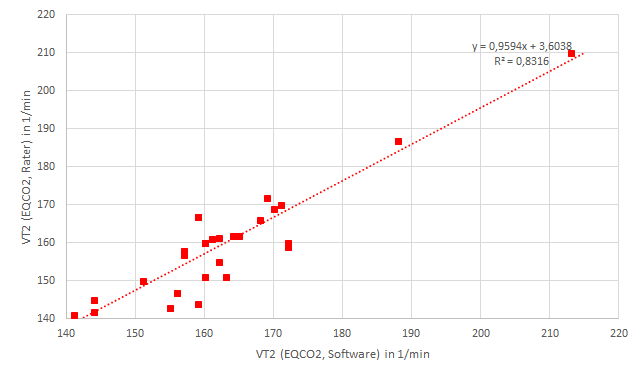
\includegraphics[scale=0.7]{Bilder/r_eqco2}
	\caption[Korrelation der \acs{EQCO2}-Ergebnisse von Ratern und Software]{Korrelation der Ergebnisse für die VT2 mit \acs{EQCO2} von Ratern und Software in Form einer Regressionsgeraden; aufgetragen wird die gemittelte VT2 gegenüber der VT2 der Software in \si{\per\minute}}
	\label{pic:pic28}
\end{figure}

Abb. \ref{pic:pic28} zeigt anhand einer Regressionsgeraden mit einem Bestimmtheitsmaß $R^2=0,83$, dass die subjektiven VT2 der Rater mit den referenzierten VT2 des Algorithmus in einen engen Zusammenhang gebracht werden können.
%
\begin{flalign*}
r_{EQCO_2} = 0,912
\end{flalign*}
%
Mit $0,912$ besitzt diese Methode im direkten Vergleich den größten Korrelationskoeffizienten.

\subsubsection{Kritische Ergebnisse}

Größere Unterschiede traten bei den Auswertungen mit \acs{VE}/\acs{VCO2} auf (siehe Abb. \ref{subpic:pic4}). Beispiele hierfür werden mit den Plots von 6w, 9m und 21m erörtert.\\
Bei Probandin 6w bestimmte Rater 1 die Schwelle im Vergleich zu Rater 2 und Software etwas früher. Abb. \ref{pic:pic17} zeigt, dass der Graph in Feld 4 von Beginn an weitestgehend linear ansteigt. Rater 1 beobachtete den ersten überproportionalen Anstieg der \acs{VE} in Stufe 5, Rater 2 und die Software erst in Stufe 7. Die Schwierigkeit bestand auch hier darin, den ersten Knickpunkt mit dem bloßen Auge zu identifizieren.\\
Abb. \ref{pic:pic19} von Proband 9m weist auch einen recht linearen Graphen in Feld 4 auf. Zudem liegen einige Messpunkte sehr dicht bei einander, was die subjektive Auswertung zusätzlich schwerer macht. Hier bestimmte der Algorithmus die VT2 eher als beide Rater.\\
Auch bei 21m unterscheiden sich die Ergebnisse von Rater 1 sowie Rater 2 und Software um eine Stufe. Abgesehen von den nicht differenzierbaren Messpunkten zwischen Stufe 3, 4 und 5, verläuft auch hier \acs{VE}/\acs{VCO2} in Feld 4 einigermaßen linear und der erste überproportionale Anstieg war der kritische Parameter.\\
Für die Auswertung von \acs{VE}/\acs{VCO2} lässt sich schlussfolgern, dass sie, ähnlich dem V-Slope, in Verbindung mit Mittelwerten und Stufentests erschwert wird, da der Graph anfällig für Artefakte ist. Eine \acs{SD} von $\pm$11 \si{\per\minute} zeigt, dass häufig keine eindeutigen Ergebnisse erzielt werden. Die Software birgt auch bei dieser Methode allerdings den Vorteil, dass die mathematische Bestimmung von Steigungsänderungen gut gelingt und die Methode somit für Vergleiche nutzbar wird. Die Ergebnisse liefern folgenden Korrelationskoeffizienten:
%
\begin{flalign*}
r_{\dot{V}E/\dot{V}CO_2} = 0,816
\end{flalign*}
%